\chapter{What is a Proof?}
\begin{pr}\leavevmode
    \begin{enumerate}[label=\textbf{(\alph*)}]
        \item \label{1.a.sec1} Colors of the triangles are arbitrary since I
        do not remember the exact ones in the text.
        \vspace{1cm}

        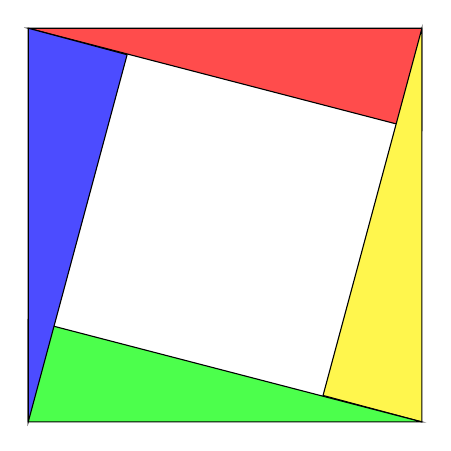
\begin{tikzpicture}
            \draw[fill=red!70] (0,0) -- (5,0) -- ++(-90:1.3) -- cycle;
            \draw[fill=yellow!70] (5,0) -- (5,-5) -- ++(165: 1.3) -- cycle;
            \draw[fill=green!70] (5,-5) -- (0,-5) -- ++(90:1.3) -- cycle;
            \draw[fill=blue!70] (0,-5) -- (0,0) -- ++(-15:1.3) -- cycle;
        \end{tikzpicture}

        \vspace{1.5\baselineskip}
        The middle square is a square of $(b-a) \times (b-a)$

        \item \label{1.b.sec1} $[$\note{Possible Errata:} Arrange the same shapes so they form
        two rectangles, both $a \times b$.$]$

        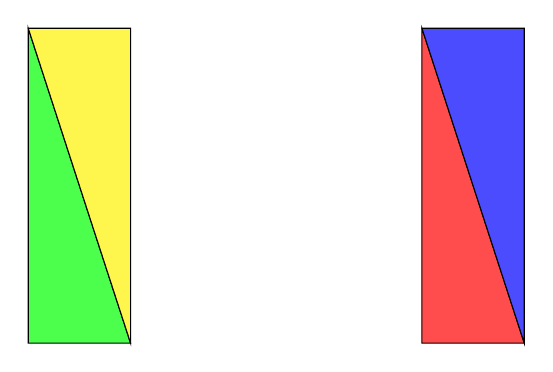
\begin{tikzpicture}
            \begin{scope}
                \draw[fill=green!70] (0,0) -- ++(0,-4) -- ++(1.3,0) -- cycle;
                \draw[fill=yellow!70] (0,0) -- ++(1.3,0) -- ++(0,-4) -- cycle;
            \end{scope}
            \begin{scope}[xshift=5cm]
                \draw[fill=red!70] (0,0) -- ++(0,-4) -- ++(1.3,0) -- cycle;
                \draw[fill=blue!70] (0,0) -- ++(1.3,0) -- ++(0,-4) -- cycle;
            \end{scope}
        \end{tikzpicture}

        We prove by construct a chain of iffs.
        \begin{IEEEeqnarray*}{C'rCl}
            & (b - a)^2 & = & c^2 - 2ab \\
            \Leftrightarrow & a^2 + b^2 - 2ab & = & c^2 - 2ab \\
            \Leftrightarrow & a^2 + b^2 & = & c^2 \\
        \end{IEEEeqnarray*}

        \item The equation would still hold true since $a = b$ is not
        a requirement for the proof. In fact, note that if $a = b$,
        the area of the bigger square in \ref{1.a.sec1} will now be
        exactly equal to the sum of area of all triangles inside it,
        which is equal to the sum of area of two smaller squares in \ref{1.b.sec1}.
        That is, $c^2 = a^2 + b^2$.

        \item Some assumptions about right triangles, squares and lines are,
        \begin{itemize}
            \item 4 identical right triangles.
        \end{itemize}
    \end{enumerate}
\end{pr}